\documentclass[11pt]{report}
\usepackage{graphicx}
\usepackage{siunitx}
\usepackage[export]{adjustbox}
\usepackage{float}
\usepackage{amsmath}
\title{EE302 Homework 4}
\date{2018\\ May}
\author{Nail Tosun - 2094563 -Section 5\\ Electric and Electronic Engineering Departmant, METU}
\begin{document}
\maketitle
\section*{Question 1}
\begin{figure}[H]
  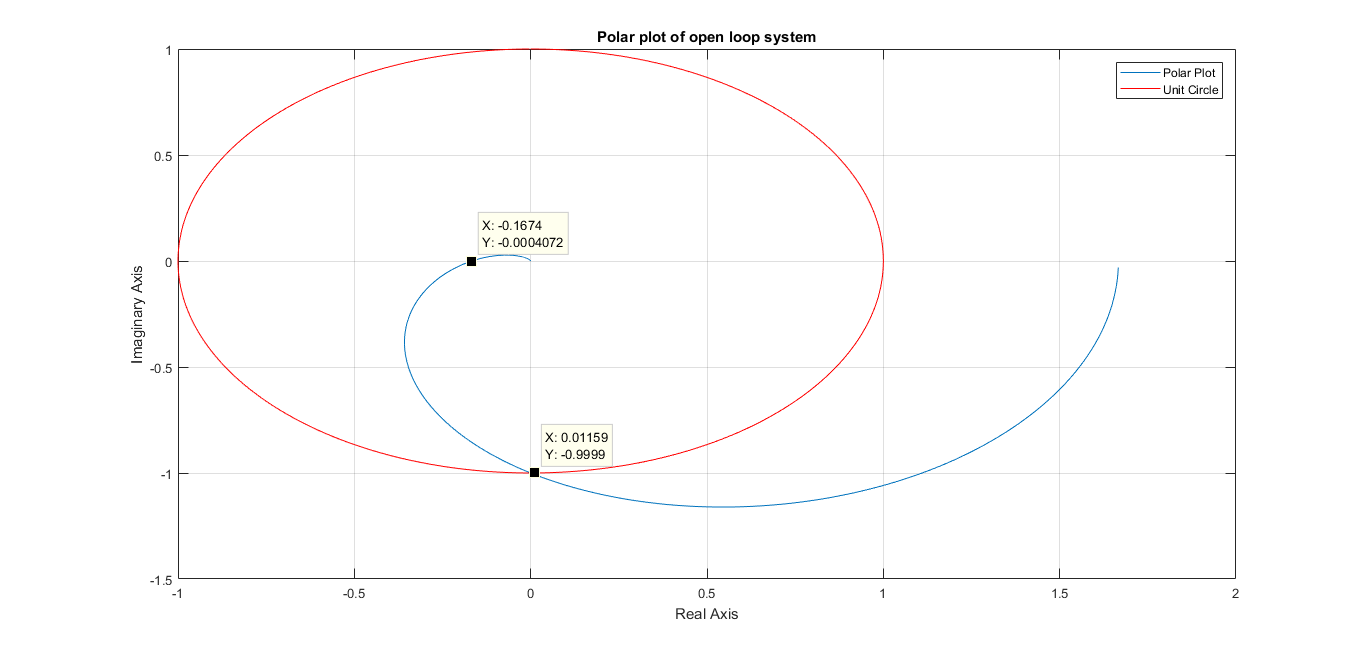
\includegraphics[scale=0.7, center]{polarplot}
  \caption{Polar plot of the system}
  \label{fig:zero}
\end{figure}
The point that cross the real axis is $x_1 = -0.1674$. Then the gain margin ;
\[GM=20log(\frac{1}{|a|})=15.5249 \>dB\]
The point where plot cross the unity circle is $x_2 =0.01159$ and $y_2=-1$. Then the phase margin is the angle between that point and the origin. 
\[PM=\ang{90}\]

\begin{figure}[H]
  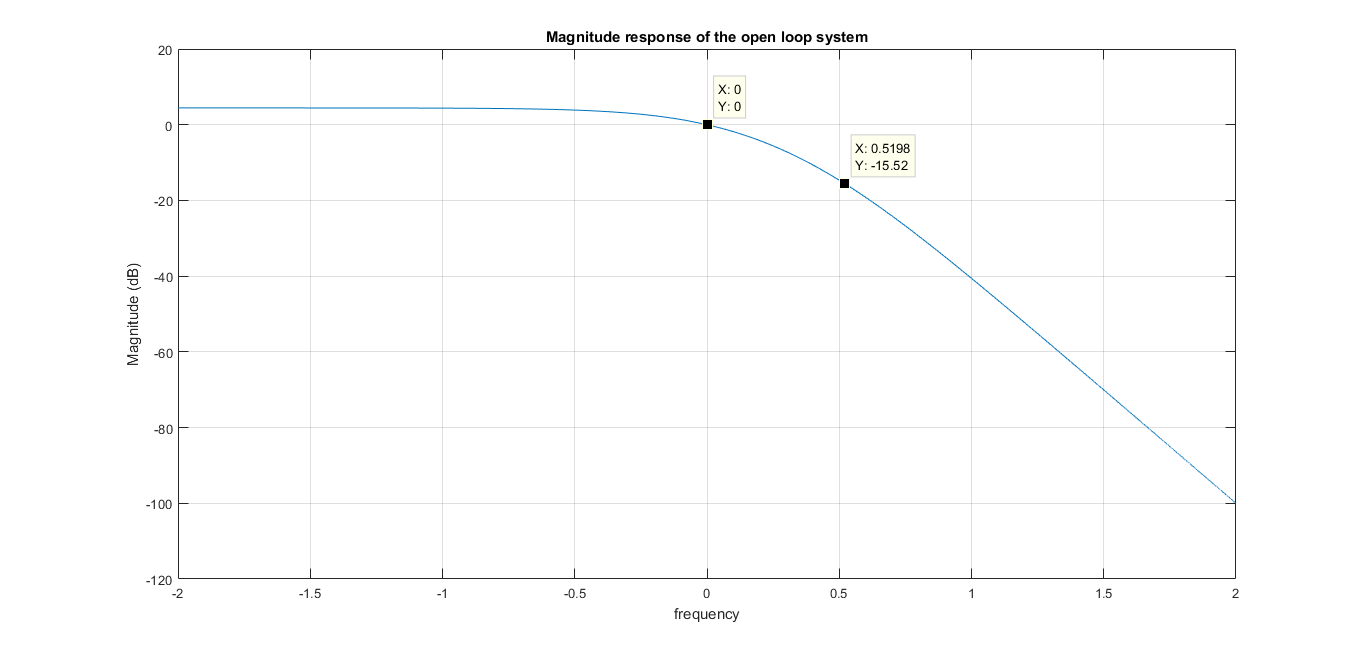
\includegraphics[scale=0.7, center]{magnitude_response}
  \caption{Magnitude response of the system}
  \label{fig:zero}
\end{figure}
Gain cross-over frequency is the frequency that system has 0 dB gain. 
\[f_{gain_{cross-over}}= 0\> \frac{rad}{sec} \> (dc)\]
To find gain margin of the system, first we find phase cross-over frequency.
\begin{figure}[H]
  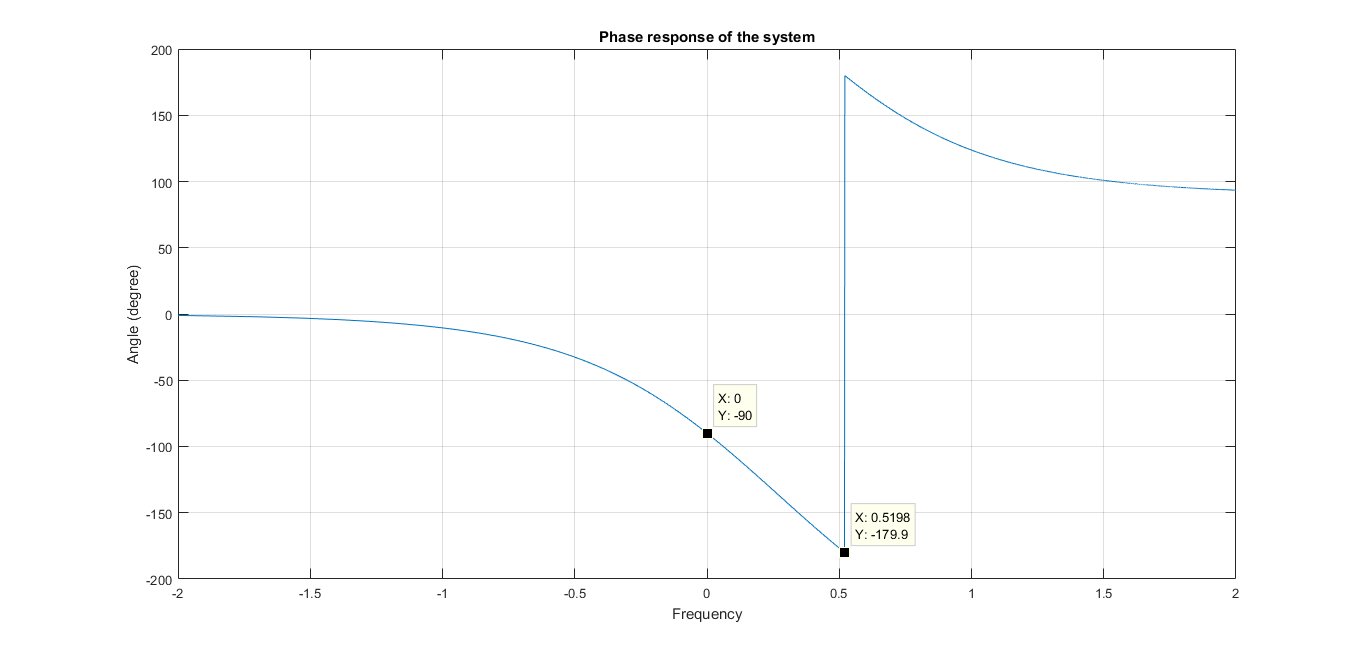
\includegraphics[scale=0.7, center]{phase_response}
  \caption{Phase response of the system}
  \label{fig:zero}
\end{figure}
\[f_{phase_{cross-over}}= 0.5198 \> \frac{rad}{sec}\]
Then the gain margin and phase margin is following
\[GM=15.52 \> dB\]
\[PM=\ang{90}\]

In both method i find exactly same gain and phase margin. 
\begin{figure}[H]
  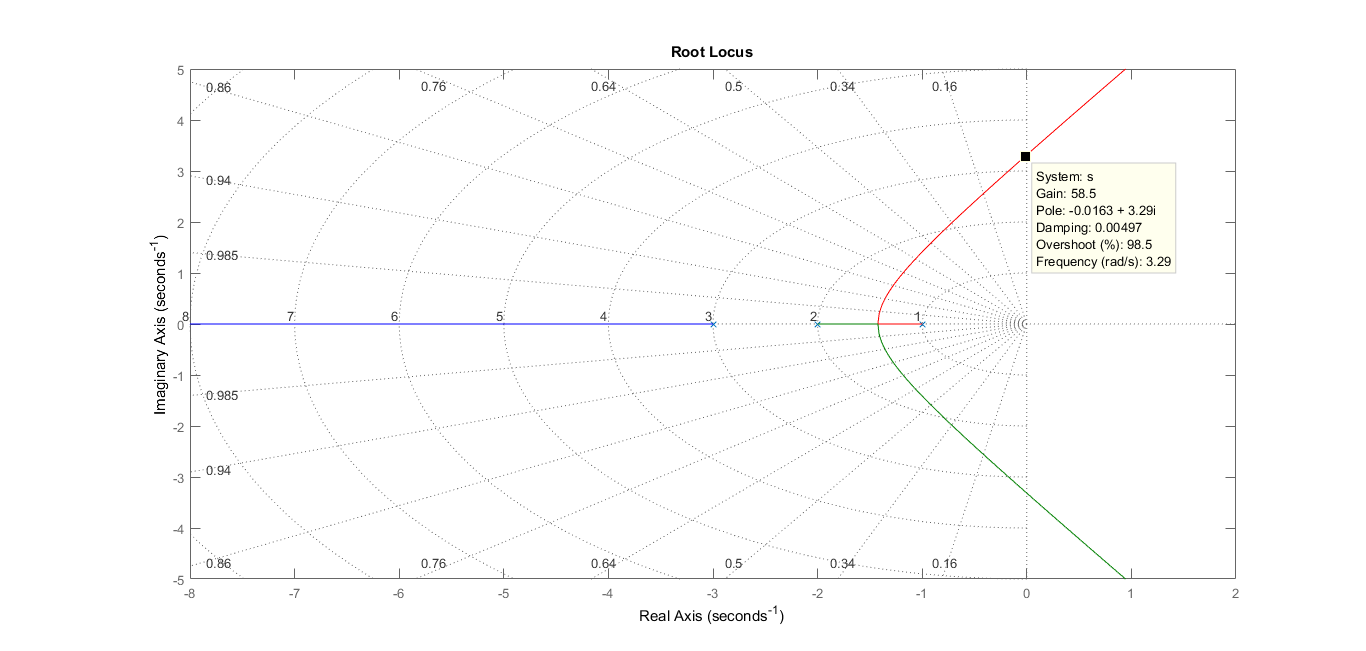
\includegraphics[scale=0.7, center]{rlocus}
  \caption{Root-locus}
  \label{fig:zero}
\end{figure}
\[K_{original}=10\]
\[K_{unstable}=58.5\]
\[GM = 20log(\frac{K_{unstable}}{K_{original}})=15.3431 \> dB\]

\section*{Question 2}
\begin{figure}[H]
  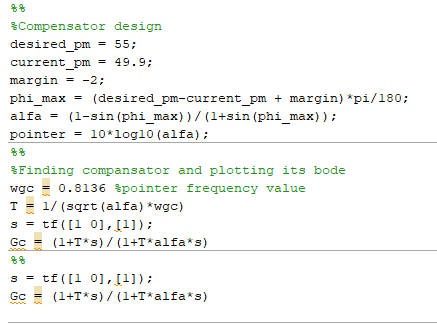
\includegraphics[scale=0.40, center]{code}
  \caption{Magnitude response of the system using experimental data}
  \label{fig:zero}
\end{figure}
\begin{figure}[H]
  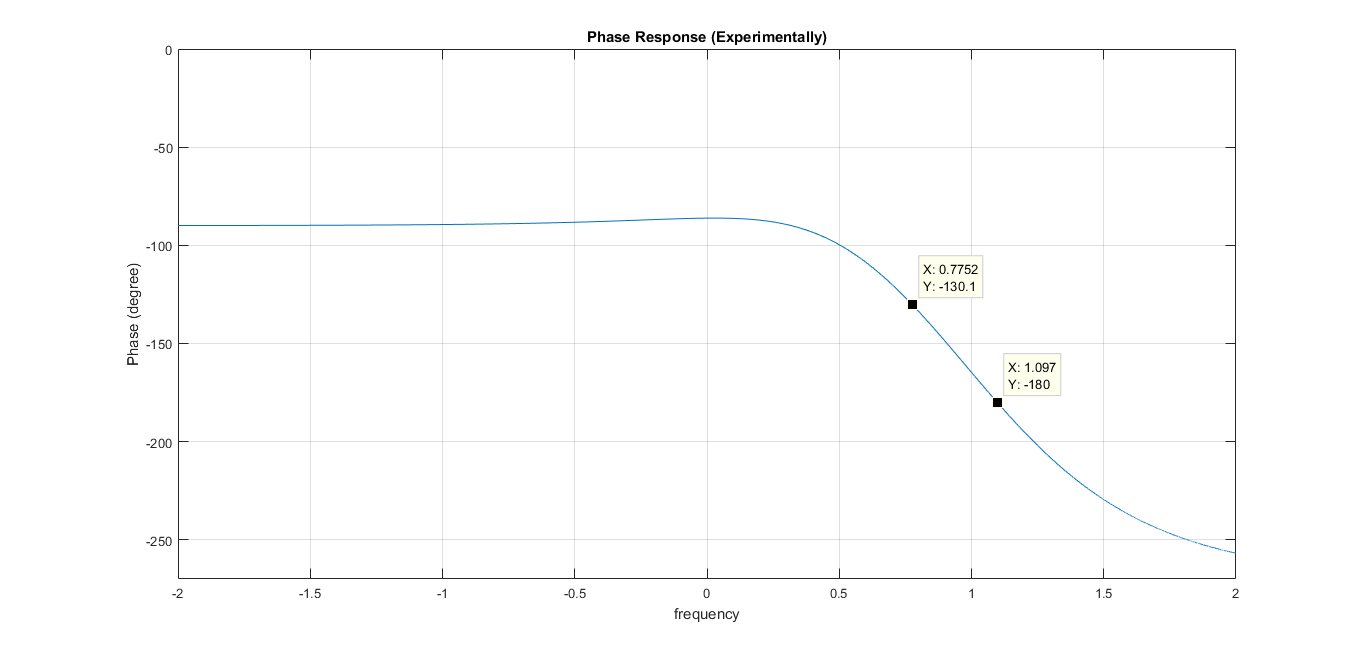
\includegraphics[scale=0.40, center]{phase_response_exp}
  \caption{Phase response of the system using experimental data}
  \label{fig:zero}
\end{figure}
\[f_{gain_{cross-over}}= 0.7752 \>\frac{rad}{sec} \>\]
\[f_{phase_{cross-over}}= 1.097 \>\frac{rad}{sec} \> (dc)\]
\[GM=10.64 \> dB\]
\[PM=\ang{49.9}\]

Transfer function of the compensator is following;
\[G_c = \frac{1+1.297s}{1+1.64s}\]

Matlab script to find its compensator parameters;

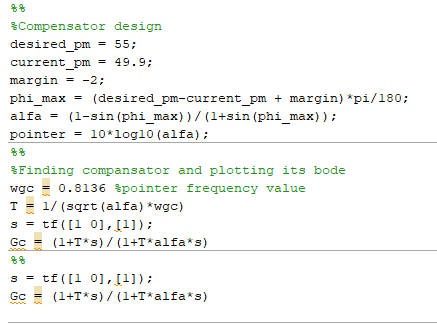
\includegraphics[scale=0.70, center]{code}
\begin{figure}[H]
\caption{Matlab script to find compensator parameters}
\label{fig:zero}
\end{figure}

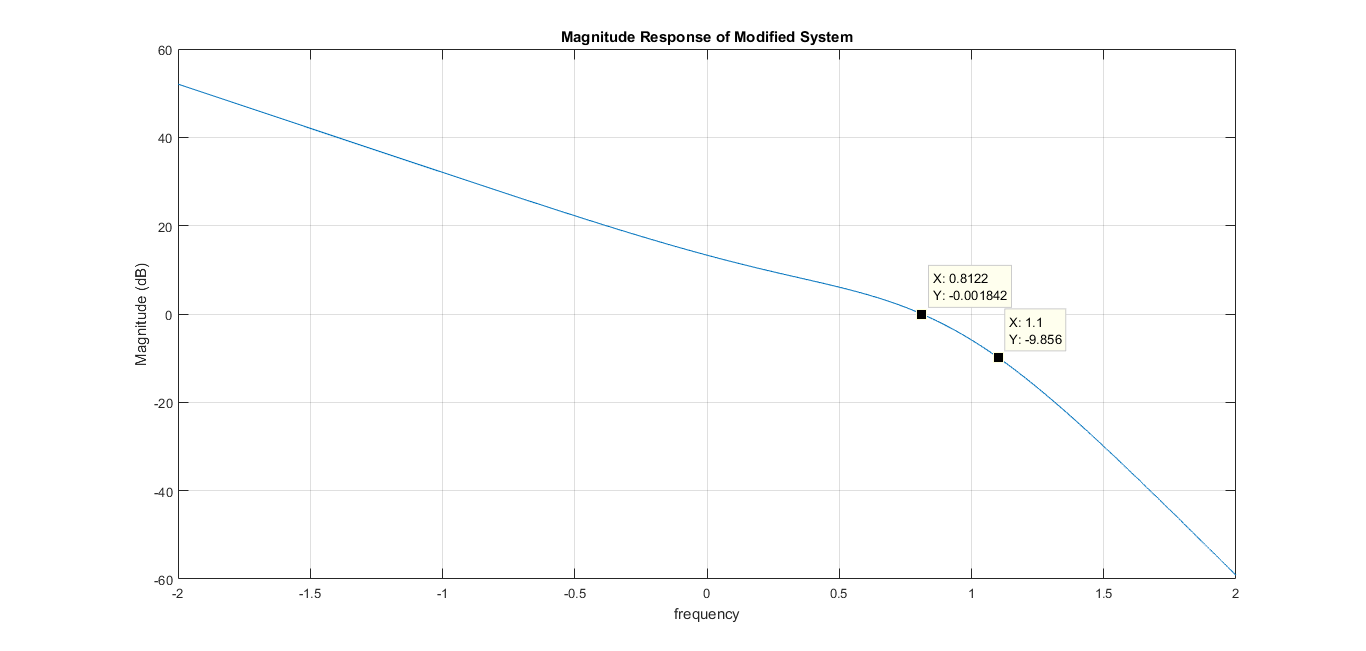
\includegraphics[scale=0.40, center]{modified_magnitude}
\begin{figure}[H]
\caption{Magnitude response of the system with lead compensator}
\label{fig:zero}
\end{figure}

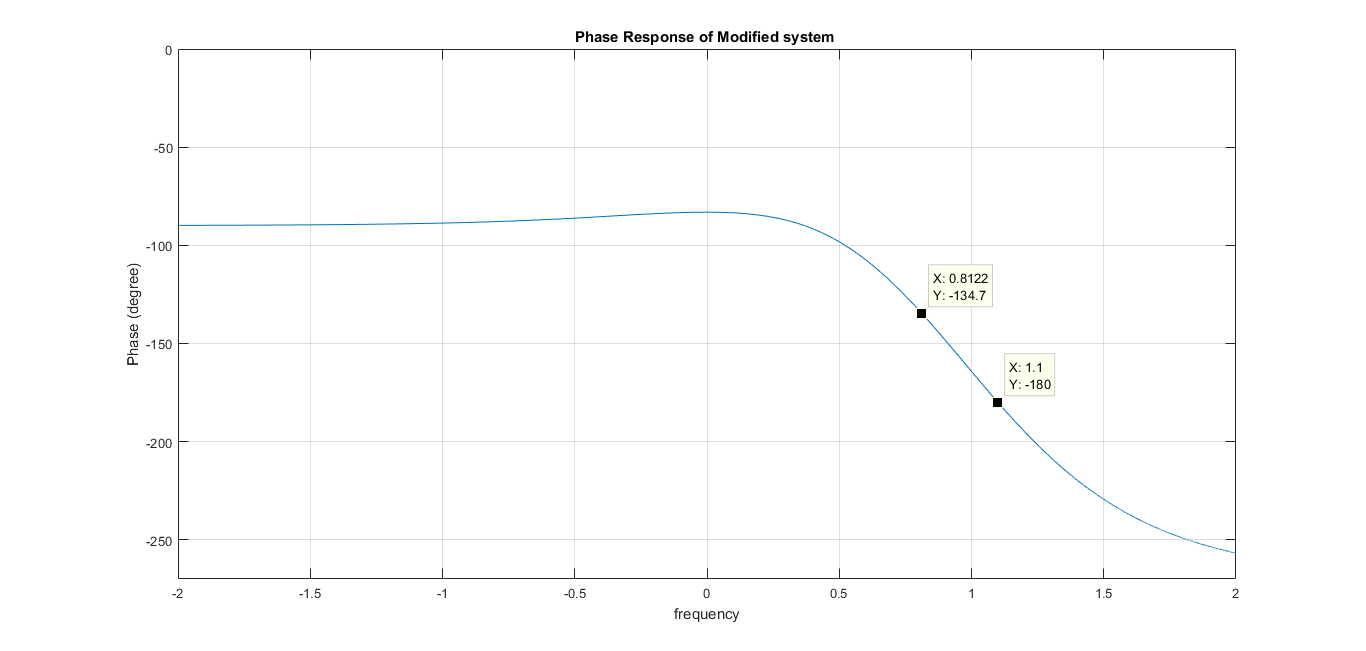
\includegraphics[scale=0.40, center]{modified_phase}
\begin{figure}[H]
\caption{Phase response of the system with lead compensator}
\label{fig:zero}
\end{figure}
\[PM=\ang{55.3}\]
\[GM=9.856 \> dB\]

Designing phase lag compensator is following;
\[\phi=-180+\phi_{desired}+5\]
From phase response desired magnitude is following
\[log(\omega_{gc})=0.5623\]
\[\omega_{gc}=3.61 \> \frac{rad}{sec}\]
\[|G(j\omega_{gc})|=4.219 \> dB \>\>\> 20log(\alpha)=4.219\> dB\]
\[\alpha=1.62\]
\[T = \frac{10}{\omega_{gc}}=2.77\]
\[T(s)=\frac{1+Ts}{1+T\alpha s} = \frac{1+2.77s}{1+4.48s}\]

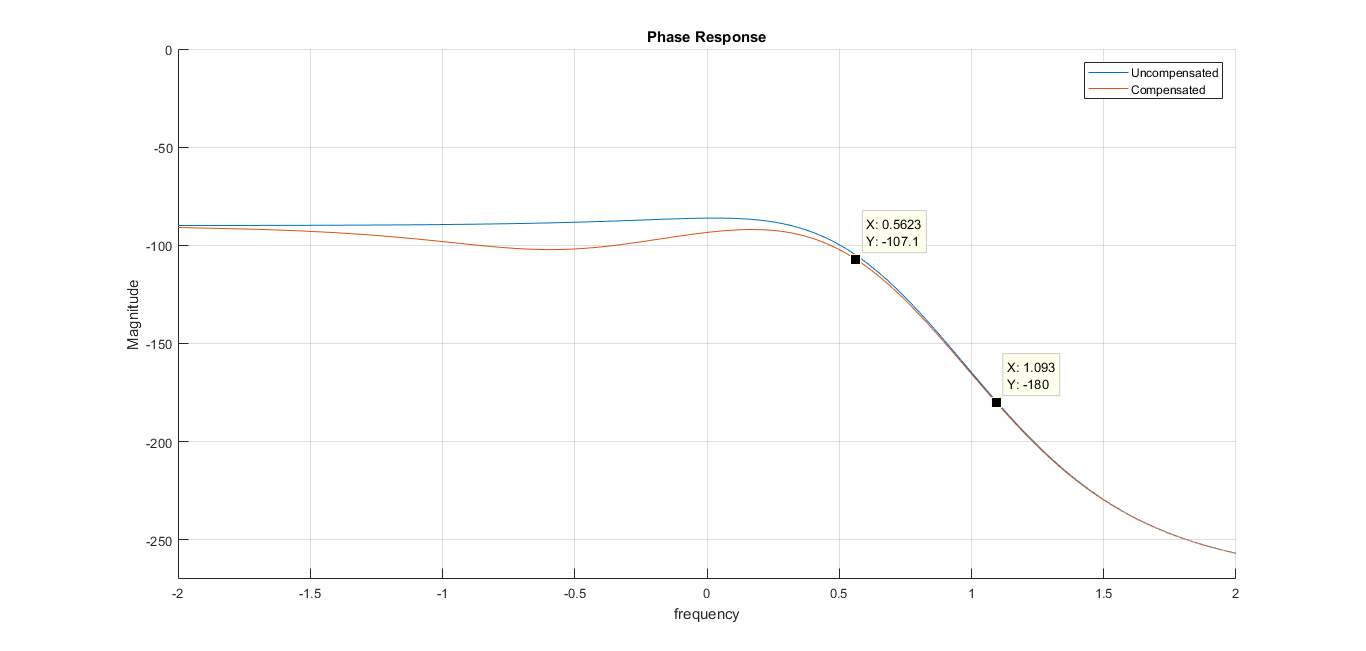
\includegraphics[scale=0.55, center]{companset}
\begin{figure}[H]
\caption{Compensated phase response}
\label{fig:zero}
\end{figure}

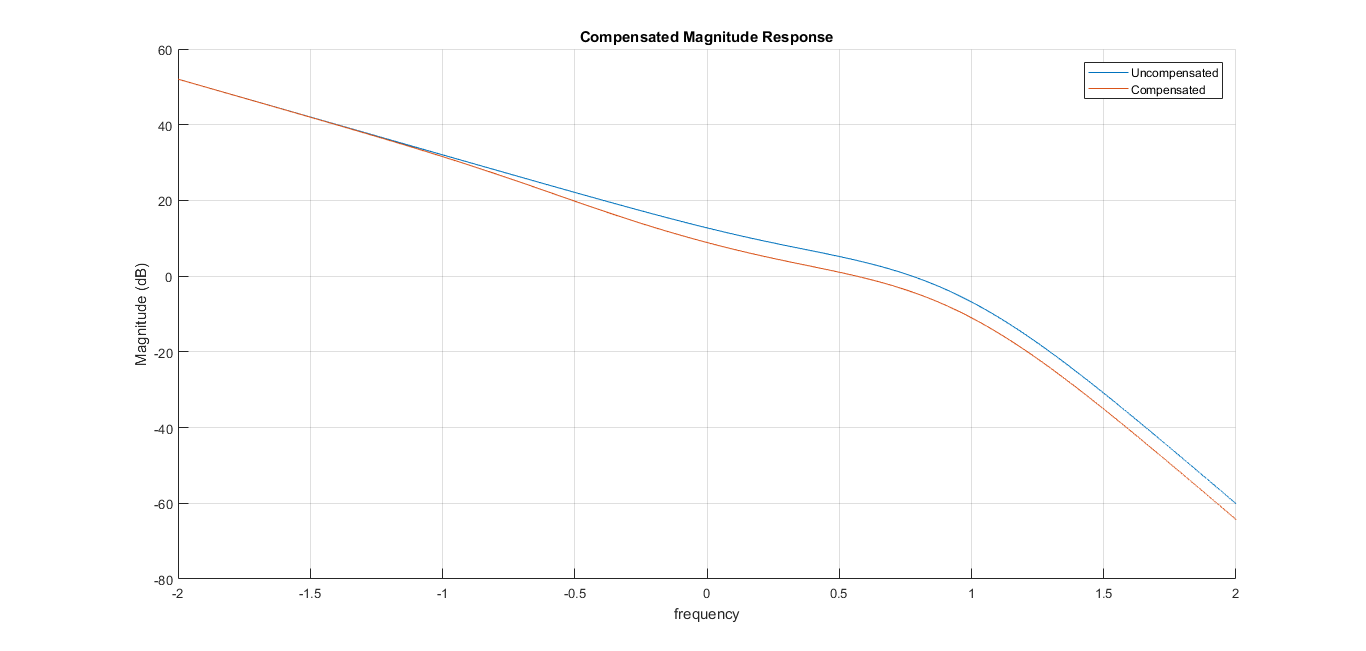
\includegraphics[scale=0.55, center]{commag}
\begin{figure}[H]
\caption{Compensated magnitude response}
\label{fig:zero}
\end{figure}

\[PM=\ang{72.9}\]
\[GM=14.69 \> dB\]
\section*{Question 3}
\[e_{ss}<0.25\]
\[G(s)=\frac{0.2}{s^2(s+100)}\]
\[K_a = \lim_{s\to 0} s^2 K G(s)\]
\[K \geq 2000\]
In order to find gain cross-over frequency following equation must solve for $\omega$;
\[G(j\omega)=\frac{(0.2)2000}{j\omega^2(j\omega+100)}=1\]
\[\omega \simeq 2 \frac{rad}{sec}\]

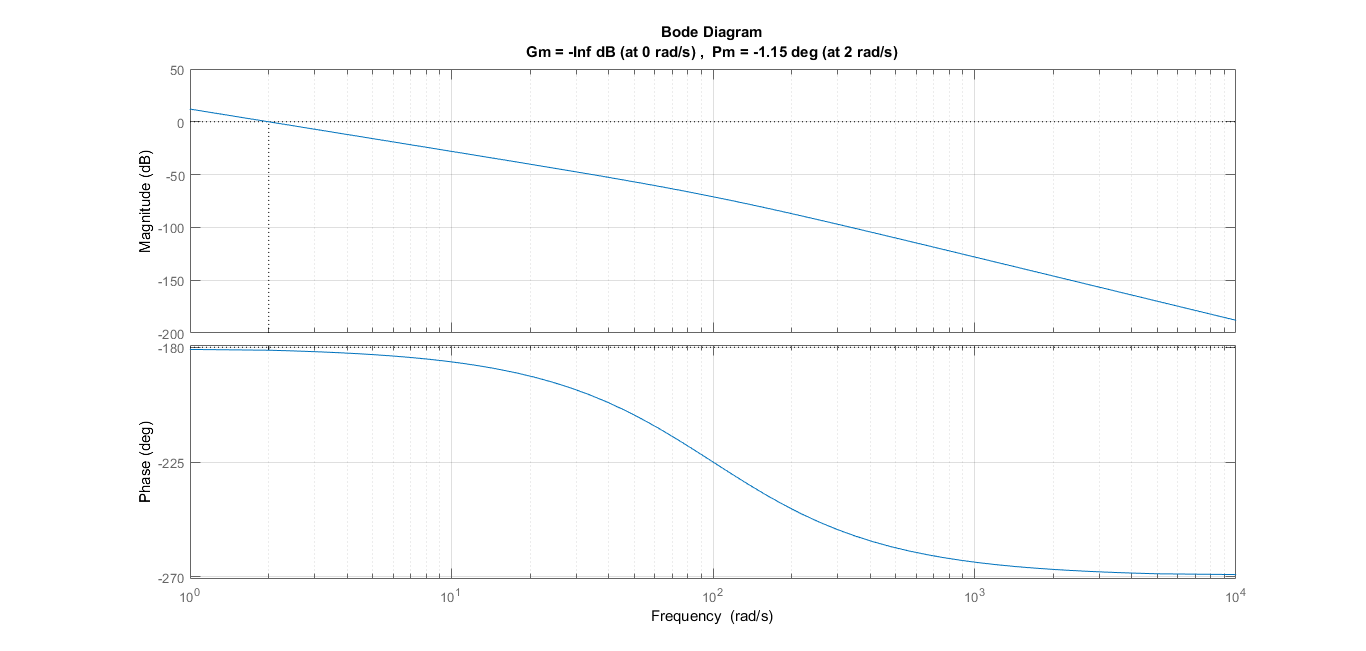
\includegraphics[scale=0.55, center]{son}
\begin{figure}[H]
\caption{Analysing circuit for compensator selection}
\label{fig:zero}
\end{figure}
Since phase margin is too low i chose lead compensator for improving phase margin. 

\[\phi_{max} = \phi_{desired} + PM + 5 \]
\[\alpha = \frac{1-sin(\phi_{max})}{1+sin(\phi_{max})} = 0.16\]
\[|G(j\omega)|=\sqrt{\alpha}=0.4\]
\[\frac{400}{\omega^2(\sqrt{10^4+\omega^2})} =0.4\]
\[\omega \simeq 3.14\]
\[T = \frac{1}{\omega \sqrt{\alpha}}\]
\[T= 0.80\]
\[G_c = \frac{1+Ts}{1+\alpha T s} = \frac{1+0.8s}{1+2.51s}\]

\end{document}